

\section{Introduction}

La DA est une technique introduite il y a une cinquantaine d'ann\'ees permettant de calculer les d\'eriv\'ees d'une fonction
 \'ecrite sous forme d'un programme source. 
Il existe deux formes diff\'erentes de DA. Soit par transformation de code, qui analyse le code original pour produire le 
code de la diff\'erenti\'ee ; le code adjoint. Il est parfois \'ecrit
\`a la main mais la DA a suffisamment fait de progr\`es pour g\'en\'erer un code en quelques minutes (pour les gros programmes) et 
d'une qualit\'e comparable d'apr\`es l'article \cite{diffautoopa}.
Soit la surcharge des op\'erateurs qui consiste \`a sp\'ecifier les calculs de 
d\'erivation associ\'es \`a chaque op\'eration effectu\'ee.
%
% explication de la diff\'erentiatation automatique : diff\'erence avec la
% diff\'erentiation symbolique et par diff\'erences finies
%

Comme indiqu\'e dans \cite{differentiaauto}, le but de la DA est de calculer la d\'eriv\'ee d'une fonction sp\'ecifi\'ee par
un programme, un algorithme. Cette m\'ethode de calcul s'oppose \`a deux autres
bien connues : la diff\'erentiation symbolique et la diff\'erentiation par
diff\'erences finies. La premi\`ere, que l'on peut retrouver dans Maple, 
utilise l'expression de la fonction pour d\'eterminer sa d\'eriv\'ee.
Cette technique est tr\`es vite limit\'ee d'une part lorsque l'on a des
expressions un peu complexes et d'autre part parce qu'il faut l'expression de la
fonction. \\
Par exemple sur Maple, si on veut obtenir :
\[\frac{\partial^3((x^2+y^2)*(\ln(x)-\ln(y)))}{\partial y \partial^2x}\]
\verb!diff((x^2+y^2)*(ln(x)-ln(y)), y,x$2);!\\
$\rightarrow$ $-\frac{2y}{x^2}-\frac{2}{y}$
\\
%

Un autre exemple de diff\'erentiation symbolique, tir\'e de \cite{Iri89onautomatic}, avec le logiciel MACSYMA \ref{fig:macsyma}

\begin{figure}
\caption{Exemple de diff\'erentiation symbolique}
\begin{center}
\fbox{
\begin{minipage}[c]{0.7\textwidth}
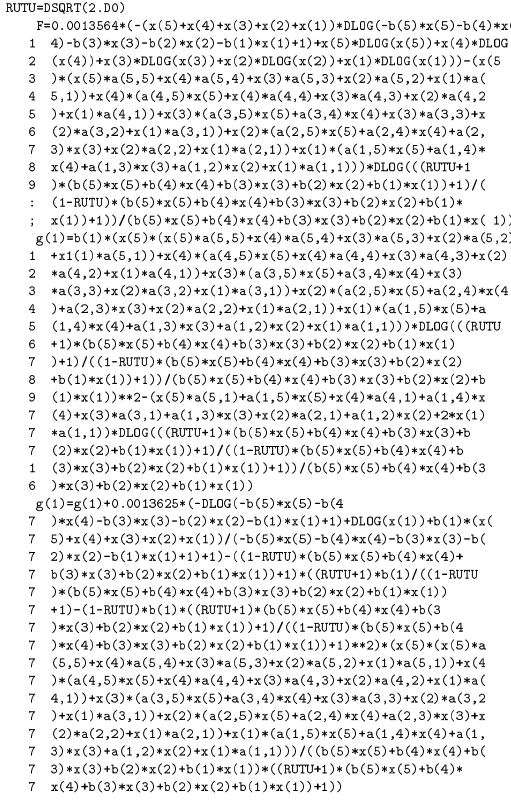
\includegraphics[scale=0.7]{figures/macsyma.png}
\end{minipage}
}
\end{center}
\label{fig:macsyma}
\end{figure}



% 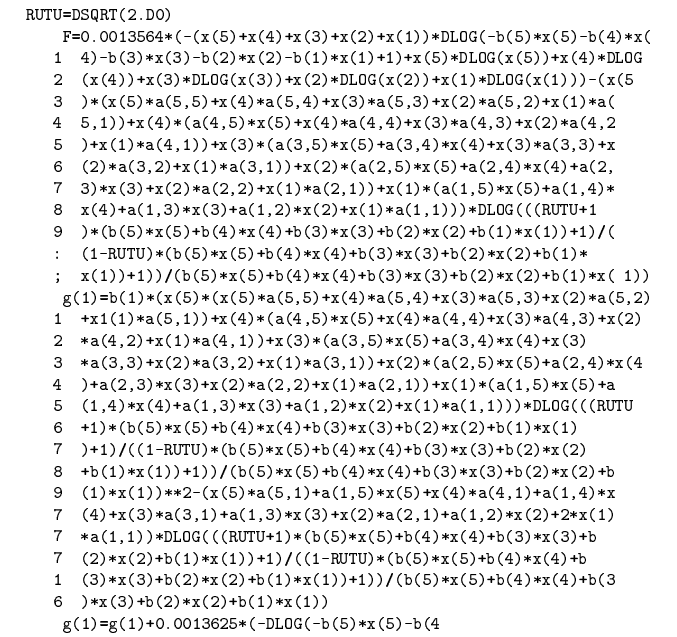
\includegraphics[scale=0.5]{figures/macsyma1.png}\\
% 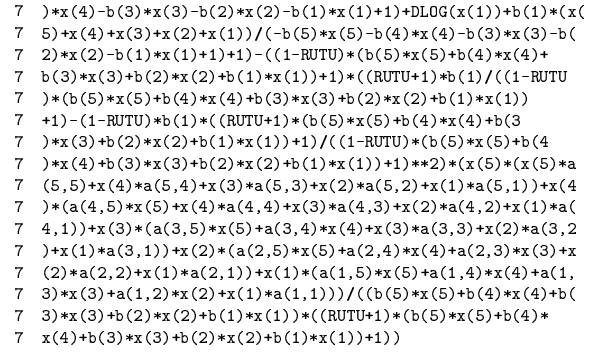
\includegraphics[scale=0.5]{figures/macsyma2.png}\\
On peut constater que l'expression devient rapidement tr\`es complexe \`a g\'erer et pas efficace.
La  plupart du temps, il faut diff\'erentier un code constitu\'e de
boucles et de conditions qui est difficilement exprimable par une expression
math\'ematique. La diff\'erentiation num\'erique ou par diff\'erences finies
s'appuie sur l'expression th\'eorique de la d\'eriv\'ee: 
$$\lim_{h\rightarrow 0}\frac{f(x+h)-f(x)}{h}$$
Dans le cas \`a plusieurs dimensions:
$$\lim_{\varepsilon \rightarrow 0}\frac{P(X+\varepsilon \cdot dX)-P(X)}{\varepsilon} =
 \nabla P(X)\cdot dX$$
Cependant, il s'agit d'un probl\`eme mal conditionn\'e \`a cause de la
discr\'etisation impos\'ee par ordinateur. $h$ doit être choisi dans l'ordre de
 grandeur de la racine de la pr\'ecision machine : si $h$ est trop proche de $0$ la
diff\'erence va être mal approch\'ee ; l'\'ecart entre $f(x+h)$ et $f(x)$
 \'etant trop faible et si $h$ est trop grand, on s'\'eloigne de la v\'eritable
valeur de la d\'eriv\'ee. Ainsi, nous allons voir que la diff\'erentiation
automatique pallie \`a ces deux inconv\'enients majeurs. \\






\section{Principes de la diff\'erentiation automatique}
\label{sec:da}



La DA calcule la d\'eriv\'ee de mani\`ere analytique, c'est-\`a-dire qu'elle obtient le calcul exact de la d\'eriv\'ee. Ainsi, il n'y a pas d'erreurs
d'approximations. \`A chaque fois qu'appara\^it une variable dans le programme source,
le programme diff\'erenti\'e va calculer une variable additionnelle de la même forme : sa diff\'erenti\'ee.
Il est \`a noter que la DA ne vise pas \`a fournir l'expression math\'ematique de la d\'eriv\'ee, puisqu'elle ne fournit que du
code permettant son \'evaluation.
Il existe deux mani\`eres d'utiliser la DA, soit le code est transform\'e pour obtenir un nouveau programme qui
calculera directement la diff\'erenti\'ee, soit par surcharge des op\'erateurs. Nous allons d\'ecrire en d\'etail ces diff\'erentes approches.
Pour la deuxi\`eme approche, il s'agit d'ajouter aux fonctions de base (l'addition, cos, log) les op\'erations de d\'erivations.




Par exemple, en prenant {\tt x}, {\tt y}, {\tt z} comme variables et {\tt V} comme vecteur,
lors de l'instruction :\\
$${\tt x= y*V(10)+z}$$\\
le programme diff\'erenti\'e va  calculer :
$$\dot{\tt x}= \dot{\tt y}*{\tt V(10)} + {\tt y}*\dot{\tt V}{\tt(10)}+\dot{\tt z} $$
en utilisant les r\`egles de d\'erivations usuelles sur les fonctions. Il n'y a plus
d'approximations, c'est un calcul exact. 
Le principe est de consid\'erer que chaque programme peut s'\'ecrire comme une s\'equence
d'instructions.
$$I_1;I_2;...;I_{p-1};I_{p}$$
Cette suite peut être identifi\'ee comme une composition de fonctions 
$$f=f_p\circ f_{p-1} \circ \cdots \circ f_1$$
par la r\`egle de d\'erivation sur la composition~(\ref{annexe:A}) on obtient :\\

\begin{align*}
f'(X) = & (f'_p\circ f_{p-1} \circ f_{p-2} \circ ... \circ f_1(X))\\
& . (f'_{p-1} \circ f_{p-2} \circ ... \circ f_1(X))\\
& \cdots\\
& . f'_1(X)\\
= & f'_p(W_{p-1}) . f'_{p-1}(W_{p-2}) . \cdots .f'_1(W_0).\\
\end{align*}
En notant $W_0=X$ et $W_k=f_k(W_{k-1})$.
%
Comme plusieurs donn\'ees sont trait\'ees, tous les $f'_k$ sont des matrices Jacobiennes de 
taille relativement grande dans un cas g\'en\'eral. Calculer la diff\'erenti\'ee revient \`a calculer
les multiplications de ces matrices. Cependant, il n'est pas possible de calculer ce produit avec un co\^ut 
raisonnable. Par exemple, avec dix variables, si on effectue une quinzaine d'instructions
cela revient \`a faire de l'ordre de $10^4$ op\'erations. La complexit\'e est exponentielle. Dans la plupart
des cas, l'application qui utilise $\nabla f(X)$  n'a en r\'ealit\'e que besoin d'une direction de la jacobienne :
 $\nabla f(X).\dot{X}$ pour une certain vecteur $\dot{X}$.
Nous allons voir les deux modes de diff\'erentiation, le mode tangent et le mode inverse. Dans le premier mode, 
les calculs de la fonctions se propagent parall\`element aux d\'eriv\'ees tandis que dans le mode inverse, le calcul
s'effectue \`a rebours en partant de la fin du code.







    \subsection{Mode tangent}

\label{chap2:tangent}
Dans notre cas, comme par exemple pour la direction de Chebychev, nous avons besoin de calculer $\nabla^3f(x)\cdot u\cdot v$ et non $\nabla^3f(x)$.
 En prenant cela en compte, le calcul va être largement simplifi\'e. \`A l'ordre un : $\dot{Y}=f'(X).\dot{X}$
$$\dot{Y}=f'_p(W_{p-1}) . f'_{p-1}(W_{p-2}) . \cdots .f'_1(W_0).\dot{X}.$$\\
Pour profiter de la multiplication avec le vecteur, le calcul va se faire de droite \`a gauche afin d'\'eviter d'avoir des multiplications de 
Matrice$\times$Matrice mais plut\^ot Matrice$\times$Vecteur. De plus, de cette mani\`ere, les appels aux $W_i$ vont
se faire dans l'ordre, donc en même temps qu'ils seront calcul\'es. Cette m\'ethode donne une combinaison lin\'eaire des 
colonnes de la matrice Jacobienne.
Voici un exemple illustr\'e pour la fonction $f(x_1,x_2)=(x_1-cos(x_2))^2$. Dans le Graphe Acyclique Orient\'e \ref{fig:gao}, le 
gradient de chaque quantit\'e en partant des feuilles va être propag\'e.


\begin{figure}
\caption{GAO : $f(x_1,x_2)=(x_1-cos(x_2))^2$ pour \'evaluer la fonction, le parcours se fait 
\`a partir des feuilles de l'arbre jusqu'\`a la racine.}
\begin{center}
\fbox{
\begin{minipage}[c]{0.45\textwidth}
\beginpgfgraphicnamed{figures/figure_14}
\endpgfgraphicnamed
\end{minipage}
}
\end{center}
\label{fig:gao}
\end{figure}




% \floatstyle{ruled}
% \newfloat{Program}{tbp}{lop}[section]
% \begin{Program}
% \begin{verbatim}
% . . . program text . . .
% \end{verbatim}
% \caption{. . . caption . . . }
% \end{Program}








\begin{figure}
\caption{GAO : mode tangent, il suit le même parcours que celui de l'\'evaluation}
\begin{center}
\fbox{
\begin{minipage}[c]{0.6\textwidth}
\beginpgfgraphicnamed{figures/figure_11}
\endpgfgraphicnamed
\end{minipage}
}
\end{center}
\label{fig:modetangent}
\end{figure}



\vspace{1cm}
\begin{tabular}{|l|c|l|c|c|}
  \hline
  $y$ & Valeurs de $y$ & $\dot{y}$ & Valeurs de $\dot{y}$ & Valeurs vectorielles
\\
  \hline
  $y_1$ &  $x_1$ &  $\dot{y_1}$ & $\dot{x_1}$ & [$1$ \ $0$] \\
  $y_2$ & $x_2$ & $\dot{y_2}$ & $\dot{x_2}$ & [$0$ \ $1$] \\
  $y_3$ & $cos(y_2)$ & $\dot{y_3}$ & $-\dot{y_2}sin(y_2)$ & -[$0$ \ $sin(x_2)$]
\\
  $y_4$ & $y_1-y_3$ & $\dot{y_4}$ & $\dot{y_1}-\dot{y_3}$ & [$1$ \ $sin(x_2)$]
\\
  $y_5$ & $y_4^2$ &  $\dot{y_5}$ & $2\dot{y_4}y_4$ & $2$[$x_1-cos(x_2)$ \
$(x_1-cos(x_2))sin(x_2)$]\\
  
  \hline
\end{tabular}



\vspace{1cm}

Le programme g\'en\'er\'e par la DA \'evalue simultan\'ement la fonction et le gradient. Le nombre de lignes obtenu
est environ deux fois celui du programme d'origine puisque chaque affectation est accompagn\'ee du calcul du
gradient. En g\'en\'eral, comme c'est expliqu\'e dans \cite{Iri89onautomatic}, le mode tangent multiplie le nombre
 d'op\'erations arithm\'etiques de $n$. Chaque quantit\'e 
$x_i$ est pr\'ec\'ed\'ee du calcul de $\nabla x_i$ de taille $n$. Dans l'exemple, on peut observer que les quantit\'es propag\'ees ont 
une dimension \'equivalente au nombre de composante de l'argument. Ainsi, le coût dû au calcul du gradient est de l'ordre de 
$n$ fois le co\^ut de l'\'evaluation de la fonction.
\vspace{0.51cm}



% \end{figure}

% 

    \subsection{Mode inverse}
Le mode inverse va nous permettre d'obtenir une ligne de la Jacobienne c'est-\`a-dire un gradient par rapport \`a 
une composante $k$.
$$\overline{X}=f'^T(X).\overline{Y}$$ 
\begin{equation}\overline{X}=f_{1}^{'T}(W_{0}) . f_{2}^{'T}(W_{1}) . \cdots .f_p^{'T}(W_{p-1}) . \overline{Y}
\label{eq:inv}
\end{equation}
L'id\'ee sous-jacente est l'utilisation des quantit\'es adjointes :

$$y_i^*= \frac{\partial f}{\partial y_i} $$
% $$y_j^*= \sum \frac{\partial f}{\partial y_j}y_i^*$$
$$\bar{y_j}= \sum_{i \in I_j} \frac{\partial f}{\partial y_j}\bar{y_i}$$
% $$\text{ o\`u tous les }\bar{y_i}\text{ sont des quantit\'es scalaires }$$
o\`u tous les $\bar{y_i}$ sont des quantit\'es scalaires
 $$I_j=\{i | y_j \text{ intervenant dans } y_i\}.$$


Le parcours du GAO se fait en profondeur, de la racine jusqu'aux feuilles. Contrairement au mode tangent,
comme les quantit\'es propag\'ees sont des scalaires, qu'une seule \'equation n'est impliqu\'ee \`a chaque n\oe ud,
 au lieu d'en avoir $n$, la dimension. Comme l'indique la figure \ref{fig:modeinverse}, les quantit\'es $\bar{y_i}$ se
propagent \`a rebours, dans le sens inverse des quantit\'es $\dot{y_i}$. C'est le fait
que le calcul se propage sur l'ensemble des feuilles qui va permettre de reconstruire le gradient de dimension $n$, chaque feuille
correspondant \`a une composante.
Commençons par observer ce mode sur notre exemple. Cette fois-ci, le parcours n'est plus le même que 
l'\'evaluation de la fonction.


\begin{figure}
\caption{GAO : mode inverse, cette fois-ci, l'arbre est parcouru depuis la racine.}
\begin{center}
\fbox{
\begin{minipage}[c]{0.75\textwidth}
\beginpgfgraphicnamed{figures/figure_12}
\endpgfgraphicnamed
\end{minipage}
}
\end{center}
\label{fig:modeinverse}
\end{figure}


\vspace{1cm}
\begin{tabular}{|l|c|}
  \hline
  $y$ & Valeurs de $y$ \\
  \hline
  $y_1$ & $x_1$ \\
  $y_2$ & $x_2$ \\
  $y_3$ & $cos(y_2)$ \\
  $y_4$ & $y_1-y_3$ \\
  $y_5$ & $y_4^2$ \\
  \hline
\end{tabular}
\hspace{1cm}
\begin{tabular}{|l|c|c|}
  \hline
 $\bar{y}$ & Valeurs de $\bar{y}$ & Valeurs \\
  \hline
 $\bar{y_5}$ & $1$ & $1$ \\
 $\bar{y_4}$ & $2y_4$ & $2(x_1-cos(x_2))$ \\
 $\bar{y_3}$ & $-\bar{y_4}$ & $2(cos(x_2)-x_1)$ \\
 $\bar{y_2}$ & $-\bar{y_3}sin(x_2)$ & $2(x_1-cos(x_2))sin(x_2)$ \\
 $\bar{y_1}$ & $\bar{y_4}$ & $2(x_1-cos(x_2))$ \\
  \hline
\end{tabular}\\

\noindent
%D'apr\`es Griewank \ref{Iri89onautomatic}, {\bf le co\^ut d'\'evaluation du gradient n\'ecessite jamais plus cinq fois le co\^ut de l'\'evaluation de la fonction}.
Dans l'\'equation \ref{eq:inv}, l'op\'eration doit se faire encore de droite \`a gauche pour que le calcul soit efficace. Malheureusement, cette fois-ci,
nous n'avons pas les appels aux $W_i$ dans le même ordre qu'ils sont calcul\'es; cela vient du fait que le parcours
n'est plus dans le même sens. Dans l'exemple, \`a la deuxi\`eme \'etape, la 
quantit\'e $y_4$ est n\'ecessaire, elle fait intervenir $y_1$ et $y_2$ alors que ces \'etats n'ont pas encore \'et\'e parcourus.
Ainsi, il existe deux strat\'egies pour obtenir les $W_i$. Soit on recalcule toutes les quantit\'es, soit on les m\'emorise toutes.




    \subsection{Strat\'egies de la DA pour le mode inverse}
% point noir stockage
% point blanc
% 
% $\overline{I_k} \rightarrow \overline{W_{k-1}}=f_k^{'T}(W_{k-1}).\overline{W_k}$
% 
\label{subsection:strategies}
 \paragraph{Recompute-All}
%  \\
Pour chaque terme $W_p=f_k(W_{p-1})$, on recalcule l'ensemble de la suite $W_i$ \`a chaque fois. L'op\'eration $W_1 =f'(X)$ va être effectu\'ee $p$ fois.
 Cette m\'ethode demande plus de temps d'ex\'ecution puisque les termes ne sont pas m\'emoris\'es, les mêmes 
calculs sont effectu\'es plusieurs fois. Les points noirs repr\'esentent le stockage de $W_k$ sur la pile
d'ex\'ecution et les points blancs repr\'esentent un d\'epilement.


% \vspace{1cm}
\begin{figure}
\caption{Strat\'egie RA : pour chaque quantit\'e \`a calculer, on reparcours le graphe pour faire un pas dans l'algorithme inverse. Prend moins de place mais
plus de temps.}
\fbox{
\begin{minipage}[c]{0.9\textwidth}
\beginpgfgraphicnamed{figures/figure_3}
\endpgfgraphicnamed
\end{minipage}
}
\label{fig:ra}
\end{figure}
% \vspace{1cm}


 \paragraph{Store-All}
Cette fois-ci, tous les termes vont être calcul\'es et enregistr\'es une seule fois. Il s'agit d'une
m\'ethode qui n\'ecessite plus de m\'emoire. Le co\^ut en m\'emoire est lin\'eaire par rapport \`a $p$.


% \vspace{1cm}
\begin{figure}
\caption{Strat\'egie SA : le graphe des \'evaluations est parcouru une seule fois pour toutes les m\'emoriser, l'algorithme inverse n'aura plus qu'\`a d\'epiler. Prend
moins de temps mais plus de capacit\'e de stockage.}
\begin{center}


\fbox{
\begin{minipage}[c]{0.9\textwidth}
\beginpgfgraphicnamed{figures/figure_4}
\endpgfgraphicnamed
\end{minipage}
}

% \beginpgfgraphicnamed{figures/figure_4}
% \endpgfgraphicnamed

\end{center}
\label{fig:sa}
\end{figure}
% \vspace{1cm}



Dans les deux cas, si le probl\`eme a une dimension trop grande, ni la strat\'egie RA, ni la SA ne pourra être
efficace. Une m\'ethode alternative appara\^it comme un bon compromis : le {\it Checkpointing}.
L'id\'ee est de d\'ecomposer le programme en plusieurs parties, si possible imbriqu\'ees et d'effectuer une sauvegarde, un {\it snapshot},
des quantit\'es entre chaque. Encore peu de travail a \'et\'e effectu\'e sur la comparaison de l'emplacement de ces {\it Checkpoints} et cela
reste une probl\`eme ouvert. Il n'y a pour l'instant pas d'emplacement optimal connu pour un algorithme quelconque. N\'eanmoins, 
ils seront \'evidemment plac\'es \`a l'ext\'erieur des sous-routines ou des boucles. \`A partir des ces 
sauvegardes on peut soit appliquer la m\'ethode RA sur la sous partie du code comme l'illustre la figure \ref{fig:checkpointra}, soit
la m\'ethode SA \ref{fig:checkpointsa}. C'est la deuxi\`eme qui a \'et\'e retenue par Tapenade car la taille de la pile est dans ce cas 
raisonnable et les ex\'ecutions d'empilement et de d\'epilement sont rapides.


\begin{figure}
\caption{Checkpoint RA - on effectue des sauvegardes \`a certains
n\oe uds du GAO et entre chacun de ces n\oe uds on adopte une strat\'egie de tout recalculer.}
\begin{center}
\fbox{
\begin{minipage}[c]{0.9\textwidth}
\beginpgfgraphicnamed{figures/figure_5}
\endpgfgraphicnamed
\end{minipage}
}
\end{center}
% \beginpgfgraphicnamed{figures/figure_5}
% \endpgfgraphicnamed
\label{fig:checkpointra}
\end{figure}
% \vspace{1cm}

\begin{figure}
\caption{Checkpoint SA - l\`a aussi, on sauvegarde les donn\'ees \`a certains n\oe uds mais entre
chaque on utilise une strat\'egie de tout m\'emoriser.}


\fbox{
\begin{minipage}[c]{0.9\textwidth}
\beginpgfgraphicnamed{figures/figure_6}
\endpgfgraphicnamed
\end{minipage}
}



% \beginpgfgraphicnamed{figures/figure_6}
% \endpgfgraphicnamed
\label{fig:checkpointsa}
\end{figure}
\vspace{1cm}




\section{Implantation de la DA}

Deux possibilit\'es s'offrent, soit la surcharge des op\'erateurs, plus flexible, soit la transformation du code.
Dans le premier cas, les op\'erateurs vont être transform\'es pour ajouter les op\'erations de d\'erivation alors que dans
la transformation du code, on ne fait qu'analyser et modifier le code texte qui permet les calculs de la fonction.

\subsection{La surcharge des op\'erateurs}

\paragraph{Programmation paresseuse}

Pour commencer \`a me familiariser avec la diff\'erentiation automatique, j'ai d'abord essay\'e de 
concevoir un programme qui d\'erive en programmation fonctionnelle. D'apr\`es l'article de Karczmarczuk \cite{paresseuse}, il est possible 
de calculer la diff\'erentiation automatique avec un langage fonctionnel de mani\`ere paresseuse.
La s\'emantique du programme original va être \'etendue par surcharge des op\'erateurs en utilisant
les r\`egles usuelles de d\'erivation. Par exemple, la r\`egle de Leibniz $(fg)'=f'g+fg'$ o\`u la r\`egle
d'encha\^inement : $(f(g(x))'=f'(g(x))g(x)$. Pour toutes op\'erations \'el\'ementaires, nous allons surcharger
par les op\'erations de d\'erivation. Pour cela, on consid\`ere une paire $(e,e')$ qui repr\'esente la valeur
orginale et sa d\'eriv\'ee. De cette mani\`ere, les constantes seront repr\'esent\'ees par $(c,0)$ et la variable
$(x,1)$. Toutes les op\'erations vont être surcharg\'ees pour ce type : $(f,f')+(g,g')=(f+g,f'+g')$, 
$(f,f')\cdot(g,g')=(f\cdot g,f'\cdot g+f\cdot g')$, $cos(f,f')=(cos(f),cos(f)\cdot f')$ et ainsi de suite.

Le langage fonctionnel que j'ai choisi est caml. On commence par d\'efinir un type expression qui traduit les op\'erations \'el\'ementaires. Comme il
 s'agit d'un exemple, la liste est non exhaustive. Le type expression est d'abord introduit, il va nous permettre d'analyser le type d'op\'eration.
En caml, il est impossible de faire un "match" sur une fonction par exemple : \begin{verbatim}| cos -> sin \end{verbatim}
c'est pour cette raison que l'on d\'efinit un constructeur de type : expression. 
{\small
\begin{verbatim}
type expression= 
    Const of float
  | Var of string
  | Opp of expression
  | Plus of expression*expression
  | Moins of expression*expression
  | Mult of expression*expression
  | Quot of expression*expression
  | Puiss of expression*float
  | Cos of expression
  | Sin of expression
  | Exp of expression
  | Log of expression
;;
\end{verbatim}
}
\noindent
Pour diff\'erentier nos constantes de nos variables, il faut introduire lors de l'\'evaluation un
environnement qui fournira la valeur de chaque variable. Par exemple si $x=3.5$ et $y=-2.1$,
$env=[("x",3.5);("y",-2.1)]$ (les parenth\`eses ne sont pas n\'ecessaires mais permettent de bien
comprendre qu'il s'agit d'une liste de couples).


Ainsi, pour \'evaluer une expression, nous n'aurons plus qu'\`a faire :

\begin{verbatim}
let rec evaluer env expr = match expr with
    Const c-> c 
  | Var v->(try List.assoc v env with Not_found ->
 raise(Unbound_variable v))
  | Opp f-> -.evaluer env f
  | Plus(f,g) -> evaluer env f +. evaluer env g
  | Moins(f,g) -> evaluer env f -. evaluer env g
  | Mult(f,g) -> evaluer env f *. evaluer env g
  | Quot(f,g) -> evaluer env f /. evaluer env g
  | Puiss(f,g) ->(evaluer env f)**g
  | Cos(f) -> cos(evaluer env f)
  | Sin(f) -> sin(evaluer env f)
  | Log(f) -> log (evaluer env f)
  | Exp(f) ->  exp (evaluer env f)
 ;;
\end{verbatim}
\noindent
{\tt List.assoc v env} permet de renvoyer l'\'el\'ement correspondant \`a {\tt v} dans la liste de couple {\tt env}. Avec notre exemple,
{\tt List.assoc "x" env} retourne {\tt 3.5}. Cette \'evaluation est la traduction du GAO. Le point apr\`es l'op\'erateur signifie que les composantes sont des {\it float}. (Les op\'erateurs
ne sont pas surcharg\'es et le \verb!+! est pour les entiers).


Pour \'evaluer la d\'eriv\'ee: 

{\small
\begin{verbatim}
let rec derive expr dv =
    match expr with
      Const c -> Const 0.0
    | Var v -> if v = dv then Const 1.0 else Const 0.0
    | Opp f -> Opp(derive f dv)
    | Plus(f, g) -> Plus(derive f dv, derive g dv)
    | Moins(f, g) -> Moins(derive f dv, derive g dv)
    | Mult(f, g) -> Plus(Mult(f, derive g dv), Mult(derive f dv, g))
    | Quot(f, g) -> Quot(Moins(Mult(derive f dv, g), Mult(f, derive g dv)),
                         Mult(g, g))
    | Puiss(f,g) -> Mult(Const g,Mult(derive f dv,f))
    | Cos(f) -> Opp(Mult(Sin(f),derive f dv))
    | Sin(f) -> Mult(Cos(f),derive f dv)
    | Exp(f) -> Mult(derive f dv,Exp(f))
    | Log(f) -> Quot(derive f dv,f)
 ;;
\end{verbatim}
}
\noindent
Karczmarczuk a propos\'e une mani\`ere d'obtenir les d\'eriv\'ees d'ordres sup\'erieurs de mani\`ere paresseuse avec Haskell,
un langage fonctionnel. La d\'efinition pr\'ec\'edente est reprise et \'etendue mais sur une liste infinie $f::f'::f''::f^{(3)}\cdots $
repr\'esentant l'expression avec l'ensemble de ses d\'eriv\'ees. 
De la même mani\`ere, les constantes seront repr\'esent\'ees par $c::0::0\cdots$
et la variable $x::1::0::0\cdots$. En notant $f=(f_0::\bar f)$ et $g=(g_0::\bar g)$ o\`u $f_0$, $g_0$ sont
les \'el\'ements en tête de liste et $\bar f$, $\bar g$ sont les listes queues, les op\'erations seront d\'efinies :
$$f+g = (f_0+g_0::\bar f+\bar g)$$
$$f\cdot g = (f_0\cdot g_0::f\cdot \bar g+\bar f\cdot g)$$
$$f/g = w \text{  o\`u  }(f_0/g_0::(\bar f\cdot g+f \cdot\bar g)\cdot w^2)$$


\noindent
On observe que la d\'efinition est auto-r\'ecursive. \'Evidemment, nous ne devrons pas \'evaluer toute la liste mais seulement les 
d\'eriv\'ees qui nous int\'eressent. Si on essaye d'obtenir {\tt w}, on boucle \`a l'infini! 
\'Etant donn\'e que caml n'est pas un langage paresseux, contrairement \`a Haskell, il a fallu construire un nouveau type que l'on 
\'evaluera uniquement quand nous en aurons besoin.


{\small
\begin{verbatim}
type 'a glacon =
| Inconnu of (unit -> 'a)
| Connu of ' a;;
\end{verbatim}
}
\noindent
Le type \verb!(unit -> 'a)! repr\'esente une fonction sans argument. Le r\'esutlat n'est que potentiellement pr\'esent; uniquement 
lorsque l'on \'evaluera cette fonction.

{\small
\begin{verbatim}
type 'a liste_paresseuse =
| Nil
| Cons of 'a cellule
and 'a cellule = { hd : 'a; mutable tl : 'a liste_paresseuse glacon};;
\end{verbatim}
}


{\small
\begin{verbatim}
let force cellule =
  let glacon = cellule.tl in
  match glacon with
  | Connu valeur -> valeur
  | Inconnu g ->
     let valeur = g () in
     cellule.tl <- Connu valeur;
     valeur;;
\end{verbatim}
}
\noindent
Forcer la cellule revient \`a \'evaluer la fonction \verb!g!.
\begin{figure}
\caption{Temps d'\'evaluation du gradient en mode direct par surcharge des op\'erateurs sur 
des listes et vecteurs avec caml}
\begin{center}
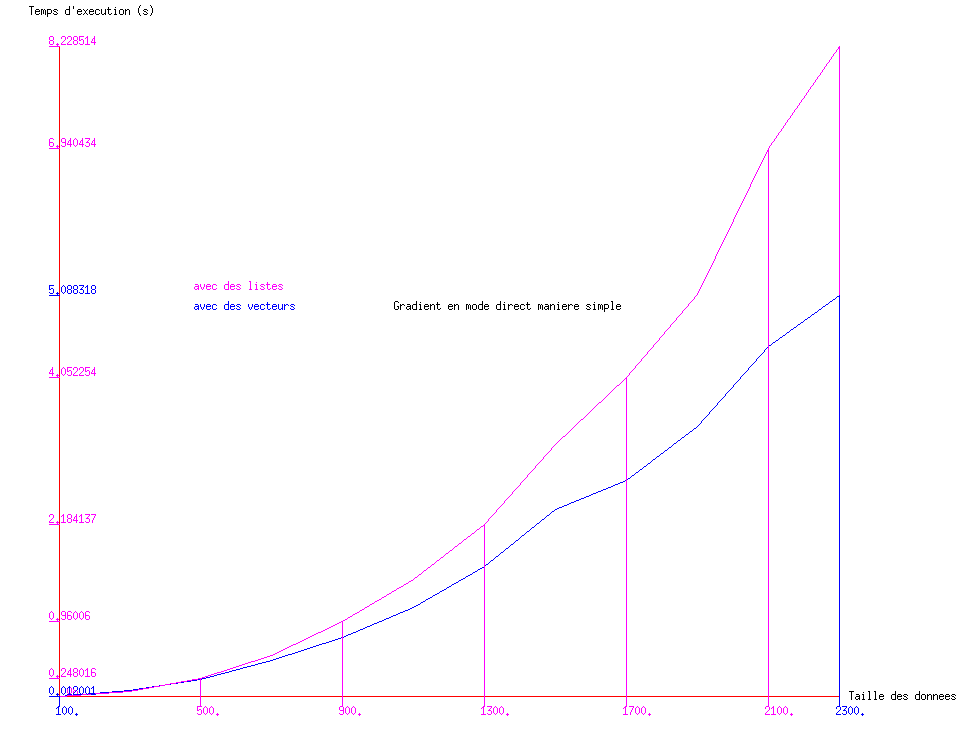
\includegraphics[scale=0.6]{figures/caml1.png}
\end{center}
\label{fig:caml1}
\end{figure}
La figure \ref{fig:caml1} illustre le fait que ces op\'erations impliquent des structures de plus en plus complexes \`a g\'erer.




On peut g\'en\'eraliser les listes infinies \`a plusieurs dimensions avec des d\'eriv\'ees partielles :
$f=(f_0,[\bar f_1,\cdots, \bar f_n] $ o\`u $\bar f_k=(\partial f/\partial f_k,[\cdots \text{ d\'eriv\'ees de }f_k' \cdots])$.
L'inconv\'enient d'une telle m\'ethode vient de la structure qui est rapidement lourde \`a g\'erer; les listes sont tr\`es dures
\`a manipuler lorsqu'elles sont de grandes tailles; $\mathcal{O}(n)$ dans le pire des cas et les vecteurs ne sont pas dynamiques.\\






\subsection{La transformation du code}
Ce proc\'ed\'e n'utilise que le code de la fonction pour g\'en\'erer celui de la d\'eriv\'ee.
Au lieu de surcharger les op\'erateurs, le code est analys\'e pour d\'etecter les variables d\'ependantes.
Ensuite, par un proc\'ed\'e analytique, il applique la d\'erivation sur les op\'erations usuelles; 
{\tt sin(x)} est transform\'ee en {\tt cos(x)*xd} o\`u {\tt xd=}$\dot x$ et il rajoute cette ligne
juste avant.

 Si on reprend le mode tangent sur notre exemple : comme variable de sortie, on a {\tt f} et 
comme variable d'entr\'ee {\tt x}.\\


{\tt
\begin{tabular}{|l|l|}
  \hline
  Code original & Mode tangent \\
  SUBROUTINE F(x, f) & SUBROUTINE F\_d(x, xd, f, fd) \\
  \hline
			& fd = xd(1) + xd(2)*SIN(x(2)) \\
    f=x(1)-COS(x(2))	& f = x(1) - COS(x(2))\\
			& fd = 2*f*fd\\
    f=f**2    		& f = f**2\\  
  \hline
\end{tabular}
}\\

Ainsi, dans le mode tangent, la valeur {\tt fd} renvoie $\nabla F(x).xd$, en scilab \\ 
{\tt derivative(F,x)*xd}.
Ce code, nomm\'e code adjoint, reste tr\`es proche du code d'origine et est imp\'eratif, contrairement \`a la surcharge d'op\'erateur qui fait 
appel \`a des fonctions r\'ecursives comme le montre l'exemple. En cela, on peut s'attendre \`a des temps d'ex\'ecution plus rapide.

Avec le mode inverse : \\

{\tt
\begin{tabular}{|l|l|}
  \hline
  Code original & Mode reverse \\
  SUBROUTINE F(x, f) & SUBROUTINE F\_b(x, xb, f, fb) \\
  \hline


     f=x(1)-COS(x(2))   &  f = x(1) - COS(x(2)) \\
     f=f**2	          &  fb = 2*f*fb \\
			  &  DO ii1=1,2 \\
			  &    xb(ii1) = 0.D0 \\
			  &  ENDDO \\
			  &  xb(1) = fb \\
			  &  xb(2) = SIN(x(2))*fb \\
			  &  fb = 0.D0 \\
			  &  END \\
  \hline
\end{tabular}
} \\
\vspace{0.5cm}
\\{\tt xb} renvoie la valeur du gradient, en scilab, {\tt xb=derivative(F,x)*fb}.



\subsection{Discussion}

La surcharge des op\'erateurs est plus souple et plus simple \`a utiliser. Il suffit en g\'en\'eral de 
d\'eclarer un nouveau type de donn\'ees.
La transformation de code source se fait en amont et utilise 
des concepts issus de la compilation en arbre de syntaxe. 


Maintenant que nous venons de voir les principes de fonctionnement, il a fallu
choisir un outil de diff\'erentiation automatique permettant d'implanter 
efficacement les op\'erations : $\nabla f$, $\nabla^2 f\cdot v$, $\nabla^2 f$, $\nabla^3 f\cdot u\cdot v$, $\nabla^3 f\cdot u$, 
$\nabla^4 f\cdot u\cdot v\cdot w$. Malgr\'e le fait 
qu'il existe actuellement plusieurs outils de DA, le choix n'est pas \'evident car pour une 
impl\'ementation efficace, il est pr\'ef\'erable d'utiliser un outil par transformation de code et 
le fait d'obtenir des d\'eriv\'ees sup\'erieures est en g\'en\'eral un point fort de la surcharge des 
op\'erateurs.
De plus, nous avons dû choisir une banque de tests ad\'equate \`a notre outil et qui repr\'esente 
suffisamment de cas de figure afin de tester correctement les algorithmes.

